\documentclass[a4paper, 12pt]{article}

%\usepackage{savetrees}
\usepackage{graphicx}
\graphicspath{{./images/}}
\title {Student Robotics 2009\\ Power Board Documentation}
\date{\today}
\setcounter{tocdepth}{1}


\begin {document}

\maketitle

\noindent This document describes the functions of the Power Board. 

\section{Board Outline}
\label{sec:outline}

\section{Functions}
\subsection{Brief Description}
The power board generates the power supplies necessary for the motors and auxiliary electronics. In addition it provides data connections to all of the Student Robotics boards, via the black, RJ11 Cables. During the competition, the power board also houses a radio module which allows your team's robot to be sent the \textit{go} and \textit{stop} commands at the beginning and end of competition rounds.

\section{Before you Begin}
You should have completed the following before beginning:
\begin{itemize}
\item	Read the Student Robotics Electronics Guidelines
\item	Charge your battery fully
\item	\ldots
\end{itemize}

\section{Assembly Instructions}
\subsection{Identify Components}
Identify the power board and orientate it with the Board Outline in section \ref{sec:outline}. A 1:1 scale drawing of the power board can be found online (http://www.srobo.org) for you to print out.

\subsection{Preparing the Connectors}
The Student Robotics modular boards are connected together using two different connectors. The black RJ11 cables (pre-assembled) are used for data whilst the green plug-in connectors are used for power. The following power connectors are provided pre-assembled:
\begin{enumerate}
\item SR Connector \(\rightarrow\) Battery (Spade sockets)
\item SR Connector \(\rightarrow\) USB Hub
\end{enumerate}

You will have to build, using the SR connectors and wire supplied, the following connectors:

\begin{enumerate}
\item Power Board  \(\rightarrow\) Motor Board
\item Power Board  \(\rightarrow\) Servo Board
\item Power Board  \(\rightarrow\) Charge-Run Switch
\item Power Board  \(\rightarrow\) Logic On/Off Switch
\end{enumerate}

\subsection{Charge/Run Switch}
This is a single-pole-double-throw switch (supplied in kit) meaning that the switch has two possible positions. You should connect this switch according to Figure \ref{fig:chrgrun}. When in charge position, the battery will charge and the motors will be \textbf{deactivated} - this is to stop the robot moving whilst plugged into the mains. In the run position, the battery \textbf{will not be charged} but the motors will be \textbf{activated}.
\begin{figure}[h!]
\center
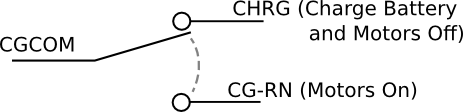
\includegraphics[scale=0.5]{chrg-run-switch}
\caption{The Charge/Run Switch}
\label{fig:chrgrun}
\end{figure}

\subsection{The On/Off switch}
Connect the single-pole-single-throw switch to the \textit{Logic Switch} indicated in the outline. This is the master power switch for your robot.

\subsection{The Powered USB Hub}
Connect the Hub's USB cable to the `Disk2' socket on the side of the slug - see figure \ref{fig:slug-side}. Now attach the SR Power \(\rightarrow\) USB Hub connector. Insert \textbf{both} memory sticks into the USB Hub.

\begin{figure}[h!]
\center
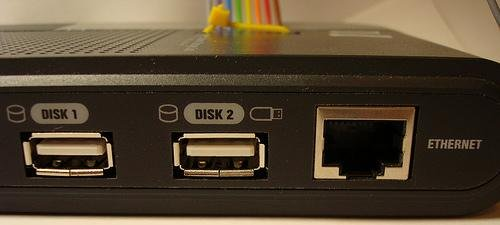
\includegraphics[scale=0.6]{slug-side-view}
\caption{Side view of the Slug's USB Ports}
\label{fig:slug-side}
\end{figure}

\subsection{The Slug}
Identify the Slug's Pin Header on the power board and \textbf{carefully} plug the Slug's multicoloured ribbon cable into it. Be sure to orientate the socket correctly, before applying force. This cable provides both power and data connections between the slug and, indirectly, all the SR modules.

\subsection{The Webcam}
Plug the USB Webcam into the spare USB port on the Slug (Disk1 in figure:\ \ref{fig:slug-side}).

\subsection{RJ11 Cables}
Connect the Motor Board, PWM Board \& JointIO Board to the Power board using three of the supplied, black, RJ11 cables. There will be a spare RJ11 socket on the power board. The order in which they are connected is unimportant. 

\subsection{Motor Board \& Servo Board Power}
Connect your SR power connector from either of the `Motor' sockets on the Power Board, to the power socket on the Motor Board. Connect another SR power connector from the `Servo' socket on the Power board, to the power socket on the PWM Board. You may have to refer to the board-specific documentation. 

These boards have different voltage requirements. Connecting them incorrectly \textbf{will damage your kit}. Be sure to check the polarity matches at both ends of the connector before proceeding to the next step.

\subsection{The Fuse}
Ensure that the fuse is fitted in the fuse socket on the power board before continuing.

\subsection{The battery}
Now attach the battery to the power board using the spade terminals spade connectors. 

\subsection{The Radio Module}
This will be supplied to you on the competition day.

\section{Powering up the slug}
To turn on your robot, ensure either charger or battery or both is connected and put the logic switch into the on position. The indicator lights on the Power board will illuminate and you will here the relay `click'. After a period of approx 20s the boot sequence will be complete, an audible beep will be heard and your robot will start executing your program code. Use the same switch to turn the robot off. 

\section{Memory Sticks}
Your team will be supplied with 2 standard USB memory sticks. One contains the operating system and files necessary for the slug to work - \textbf{do not overwrite this USB stick}. The second stick contains your program code and can be rewritten by checking out your code from the Student Robotics IDE and copying the generated zip file to it.

\section{Trouble shooting}
\subsection{No lights illuminate}
Is the fuse fitted and not blown? Is the battery or charger connected? Is the battery charged?
\subsection{The Slug never boots/beeps}
Are both memory sticks plugged in to the USB Hub? Is the USB Hub powered?
\section{Glossary}
\begin{tabular}{| l | p{5cm}|}
\hline
SR Connector & Green 2-Way or 3-Way plug-in male connector with screw terminals. \\ \hline
Battery Connector & 2.1mm jack \\
\hline
\end{tabular}
\end {document}
